% This is "sig-alternate.tex" V2.1 April 2013
% This file should be compiled with V2.5 of "sig-alternate.cls" May 2012
%
% This example file demonstrates the use of the 'sig-alternate.cls'
% V2.5 LaTeX2e document class file. It is for those submitting
% articles to ACM Conference Proceedings WHO DO NOT WISH TO
% STRICTLY ADHERE TO THE SIGS (PUBS-BOARD-ENDORSED) STYLE.
% The 'sig-alternate.cls' file will produce a similar-looking,
% albeit, 'tighter' paper resulting in, invariably, fewer pages.
%
% ----------------------------------------------------------------------------------------------------------------
% This .tex file (and associated .cls V2.5) produces:
%       1) The Permission Statement
%       2) The Conference (location) Info information
%       3) The Copyright Line with ACM data
%       4) NO page numbers
%
% as against the acm_proc_article-sp.cls file which
% DOES NOT produce 1) thru' 3) above.
%
% Using 'sig-alternate.cls' you have control, however, from within
% the source .tex file, over both the CopyrightYear
% (defaulted to 200X) and the ACM Copyright Data
% (defaulted to X-XXXXX-XX-X/XX/XX).
% e.g.
% \CopyrightYear{2007} will cause 2007 to appear in the copyright line.
% \crdata{0-12345-67-8/90/12} will cause 0-12345-67-8/90/12 to appear in the copyright line.
%
% ---------------------------------------------------------------------------------------------------------------
% This .tex source is an example which *does* use
% the .bib file (from which the .bbl file % is produced).
% REMEMBER HOWEVER: After having produced the .bbl file,
% and prior to final submission, you *NEED* to 'insert'
% your .bbl file into your source .tex file so as to provide
% ONE 'self-contained' source file.
%
% ================= IF YOU HAVE QUESTIONS =======================
% Questions regarding the SIGS styles, SIGS policies and
% procedures, Conferences etc. should be sent to
% Adrienne Griscti (griscti@acm.org)
%
% Technical questions _only_ to
% Gerald Murray (murray@hq.acm.org)
% ===============================================================
%
% For tracking purposes - this is V2.0 - May 2012

\documentclass{sig-alternate-05-2015}
%\pagestyle{plain}

\usepackage{algorithm}
\usepackage{algpseudocode}


\begin{document}

% Copyright
\setcopyright{acmcopyright}
%\setcopyright{acmlicensed}
%\setcopyright{rightsretained}
%\setcopyright{usgov}
%\setcopyright{usgovmixed}
%\setcopyright{cagov}
%\setcopyright{cagovmixed}

\pagenumbering{arabic}

% DOI
\doi{}

% ISBN
\isbn{}

%Conference
\conferenceinfo{}{Feb 25, 2015}

%
% --- Author Metadata here ---
\conferenceinfo{}{}
%\CopyrightYear{2007} % Allows default copyright year (20XX) to be over-ridden - IF NEED BE.
%\crdata{0-12345-67-8/90/01}  % Allows default copyright data (0-89791-88-6/97/05) to be over-ridden - IF NEED BE.
% --- End of Author Metadata ---
\title{Music Recommender and Genre classification system}
\subtitle{}
%
% You need the command \numberofauthors to handle the 'placement
% and alignment' of the authors beneath the title.
%
% For aesthetic reasons, we recommend 'three authors at a time'
% i.e. three 'name/affiliation blocks' be placed beneath the title.
%
% NOTE: You are NOT restricted in how many 'rows' of
% "name/affiliations" may appear. We just ask that you restrict
% the number of 'columns' to three.
%
% Because of the available 'opening page real-estate'
% we ask you to refrain from putting more than six authors
% (two rows with three columns) beneath the article title.
% More than six makes the first-page appear very cluttered indeed.
%
% Use the \alignauthor commands to handle the names
% and affiliations for an 'aesthetic maximum' of six authors.
% Add names, affiliations, addresses for
% the seventh etc. author(s) as the argument for the
% \additionalauthors command.
% These 'additional authors' will be output/set for you
% without further effort on your part as the last section in
% the body of your article BEFORE References or any Appendices.

\numberofauthors{3} %  in this sample file, there are a *total*
% of EIGHT authors. SIX appear on the 'first-page' (for formatting
% reasons) and the remaining two appear in the \additionalauthors section.
%
\author{
% You can go ahead and credit any number of authors here,
% e.g. one 'row of three' or two rows (consisting of one row of three
% and a second row of one, two or three).
%
% The command \alignauthor (no curly braces needed) should
% precede each author name, affiliation/snail-mail address and
% e-mail address. Additionally, tag each line of
% affiliation/address with \affaddr, and tag the
% e-mail address with \email.
%
% 1st. author
\alignauthor
Sunil BN\titlenote{Graduate Student}\\
       \affaddr{University of Colorado Boulder}\\
       \affaddr{Boulder, Colorado}\\
       \affaddr{United states}\\
       \email{suba5417@colorado.edu}
% 2nd. author
\alignauthor
Praveen Kumar Devaraj\titlenote{Graduate Student}\\
       \affaddr{University of Colorado Boulder}\\
       \affaddr{Boulder, Colorado}\\
       \affaddr{United states}\\
       \email{prde1873@colorado.edu}
% 3rd. author
\alignauthor
Suresh Kumar\titlenote{Graduate Student}\\
       \affaddr{University of Colorado Boulder}\\
       \affaddr{Boulder, Colorado}\\
       \affaddr{United states}\\
       \email{suku3476@colorado.edu}
}
% There's nothing stopping you putting the seventh, eighth, etc.
% author on the opening page (as the 'third row') but we ask,
% for aesthetic reasons that you place these 'additional authors'
% in the \additional authors block, viz.

% Just remember to make sure that the TOTAL number of authors
% is the number that will appear on the first page PLUS the
% number that will appear in the \additionalauthors section.

\maketitle
\begin{abstract}
In the recent years, music recommendation systems are gaining popularity because a lot of music is now sold digitally. Most of the music recommender system are based on collaborative filtering or content based filtering. This project presents a hybrid music recommendation method that solves two of inherent problems in conventional methods. Collaborative approach cannot recommend music that has no ratings and suffers from cold start. The aim is to recommend a list of songs to a user given a little about his/her listening history and complete listening history of other 1 million users. Where as content based filtering recommends music based on the similarity of contents and doesn't truly reveal the user preferences.

Our approach combines both methods i.e based on user rating and content using discriminative model. We propose to train the collaborative filtering model such as Mlib (Machine learning library) and predict songs user might be interested in and over which we run the content based filtering in order to make the recommendations more accurate and closer to the user preferences.

We propose to try different classification techniques in content based filtering to generate a comparison of the efficacy of each of the techniques in the prediction a list that is closest to the user preferences. We compare a few conventional methods of collaborative and content based filtering with our hybrid model, and evaluate the predictions quantitatively and qualitatively on the Million Song Data-set(MSD).

\end{abstract}


% We no longer use \terms command
%\terms{Theory}

\keywords{Hybrid model; collaborative filtering; content based filtering; Machine learning library(Mlib); Million song dataset, MSD}

\section{Motivation}
Given a huge collection of digital media like audio, video etc a recommender system help users find and select items of their tastes. The Music recommender system will present to the listeners a subset of the songs that are well suited to their interest based on mood/genre/time of day etc. Thus building a robust music recommendation and Genre classification system is complicated by the variety of songs, lyrics, content of the songs and size of dataset etc. There is no single solution that can be classified as the best solution for the recommendation as a lot of factors determine the liking of a song by the user.

Further more most of the recommendation system work on either collaborative or content based filtering, both have their pros and cons.

Collaborative Filtering recommend songs to the user by considering how other users have rated them. In this case those songs which have not been rated are not considered which reduces the training data to a large extent. Also this depends on the user preferences, the artists of the recommended pieces could be the same and most users tend to rate their songs highly. So the recommendations made are unrelated to the user preferences.
 
Content-based methods recommend songs similar to the users' listening history in terms of musical properties. This results in a large variety of artists i.e. various songs are recommended even when they have not been rated. However, these methods have low accuracy of recommendations because similarity in content is only one of many factors characterizing user preferences.

Thus, in this project we will consider best features of both the conventional methods to build a better and more accurate music recommender system and also compare this with the existing recommender systems.


\section{Literature Survey}
With the explosion of Internet in recent decades, Internet has become a major source for information such as audio, video, books, geography etc. The music also has drifted more and more towards the digital distribution of musical pieces through on-line stores like iTunes, Spotify, SoundCloud, Shazam and Google play music. As a result music categorization and recommendation has become a persistent problem. Music categorization allow on-line music to be classified based on the genre, lyrics etc. so that the users' can browse through the similar contents. And recommender system enables users' to discover new music that matches their tastes based on previously listened music.\\

Though much of the studies and research has been done in recommender system, still the problem here is complicated by the variety of tons of songs, different genres, social and geographical factors that influence the users. The number of music that can be recommended to the user is very large.\\

The problem is to organize the humongous amount of music available on-line into categories like based on genre, artist, most popular etc.MIR  techniques  have  been  developed  to  solve problems  such  as  genre  classification,  artist  identification,  and  instrument recognition. Since 2005, an annual evaluation event called Music Information Retrieval Evaluation eXchange (MIREX1) is held to facilitate the development of MIR algorithms\cite{DeepContentbased}.\\

Additionally, music recommender system is to help the users find and discover the music according to their tastes. A good recommender system should be able to learn the listening styles/preferences of users and generate play-list accordingly. Meanwhile, the development of recommender systems provides a great opportunity for industry  to  aggregate  the  users  who  are  interested  in  music.  More  importantly, it raises challenges for us to better understand and model users preferences in music.\\

Some music discovery websites such as Last.fm, Allmusic, Pandora and Shazam have successfully used these two approaches into reality. In the meantime, these websites provide an unique platform to retrieve rich and useful information for user studies.\\

\section{Proposed work}
The two main objective of the project is to recommend songs to users and genre classification of songs.

\subsection{Building a Music Recommender System}

There are three approaches to building a recommender system - Collaborative filtering, Content-based filtering and a hybrid approach. Each of these approach makes use of users and items data. In this paper, we use the term items and songs interchangeably. The following section describes each approach. For the project, we will use a hybrid approach combining collaborative filtering and content based filtering techniques.

\subsubsection{Collaborative Filtering Approach}

The first approach is to recommend songs using collaborative filtering (CF) technique. Collaborative filtering is based on the idea of determining user's preference using the listeners' historical data. Collaborative filtering technique recommends a song to the test user based on how other users rated the recommended song. For example, if a user listened to song A, B, C and another user listened to song B, C, D then song D would be recommended to 1st user and song A would be recommended to the second user. \\\\
There are two types of collaborative filtering approaches:  Memory based and Model-Based. Memory based approach uses user rating data to compute the similarity between the users or the songs. Memory based approach is easy to implement but its performance decreases as the data gets sparse which is quite the case with our songs database. \\
A popular way to compute the similarity between two users $x$ and $y$ is to use the cosine similarity where $I_{xy}$ is the set of items rated by both users $x$ and $y$:
\begin{equation*}
    sim(x, y) = cos(x, y) = \frac{\sum_{i \in I_{xy}}^{} r_{x,i} r_{y,i}}{\sqrt{\sum_{i \in I_{xy}}^{} r_{x,i}}\sqrt{\sum_{i \in I_{xy}}^{} r_{y,i}}}
\end{equation*}

\\
Model bases approach uses data mining techniques and machine learning algorithms to find patterns based on training data. The users and items are described by a small set of latent factors that can be used to predict missing entries. This technique handles sparsity better, is scalable with large dataset and improves prediction performance. We will consider model-based approach to CF and make use of the Alternating Least square algorithm to learn the latent factors. The play count of a song will be used as the rating value.\\

The low-rank matrix factorization is a minimization problem, in which the cost function measures the fit between a given matrix (user preference matrix) and an approximating matrix, subject to a constraint that the approximating matrix has reduced rank.
\begin{figure}[h]
    \centering
    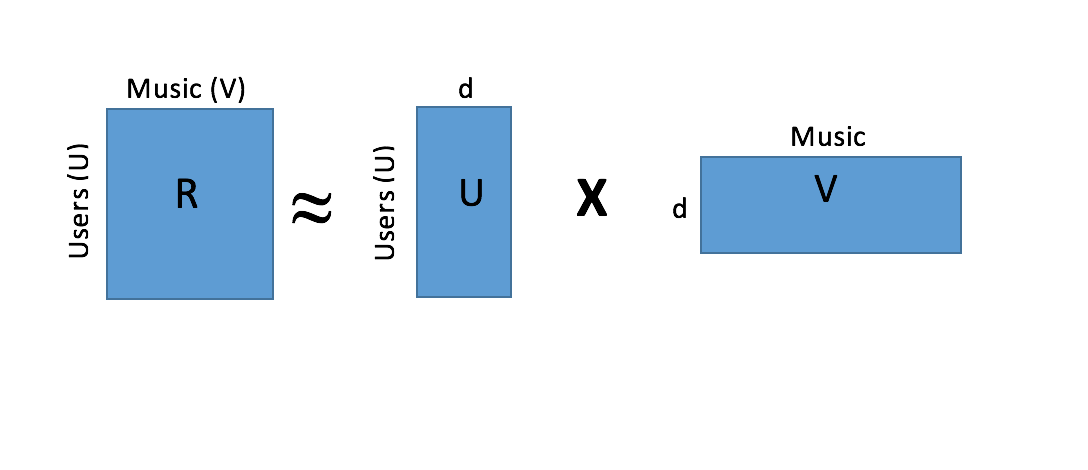
\includegraphics [width =10cm]{Images/LRMFactorization.png}
    \caption{Low Rank Matrix Factorization}
\end{figure}

The low rank approximation problem is thus formulated as follows to learn the factor vectors $(u_i, v_j)$,
\begin{equation*}
   (u_i, v_j) = \min_{x, y}\sum_{(u,i)\in K}^{} (p_{u,v}-r_{u,v})^2
\end{equation*}
where, $p_{u,v}$ and $r_{u,v}$ are predicted and observed ratings for user $u$ and item $v$ respectively. $K$ is a sparse matrix of known ratings.\\\\
Solving the low rank approximation problem as formulated above usually overfits the data. In order to avoid overfitting a common technique is to use Tikhonov regularization to transform the low rank approximation problem into the following:
\begin{equation*}
   (u_i, v_j) = \min_{x, y}\sum_{(u,i)\in K}^{} (p_{u,v}-r_{u,v})^2 + \lambda(||u_i||^2+||v_j||^2)
\end{equation*}
where, $\lambda$ is regularization parameter, which penalizes parameters with large magnitude.
\\
\begin{algorithm}
\caption{ALS Algorithm}
\label{CHalgorithm}
\begin{algorithmic}[1]
\State Set up vectors yUsers, yItems, xq, and xp
\State Initialize $\mu$, $a_i$, $b_u$, $y_{ui}$
\While{MSE not converged and iteration $\ne$ max limit}
\State Create $q_i$ vectors
\State    Solve for $p_u$ vectors 
\State Create $p_u$ vectors
\State    Solve for $q_i$ vectors
\State Rescale each $p_u$ and $q_i$ vector 
\State Update $\mu$, $a_i$, $b_u$, $y_{ui}$
\State Find MSE
\EndWhile
\end{algorithmic}
\end{algorithm}

\\\\\\
The advantage of Collaborative filtering approach is that it does not need to have any information about the songs. The key issue with this approach is that is needs to have a large user data and thus suffer from cold start state for new users or new items. In order to make appropriate recommendations for a new user, the system must first learn the user preference by analyzing rating activities. This method cannot recommend new song releases, i.e., the songs which has never been listened by any user in the database.\\\\\\
\begin{figure}[h]
    \centering
    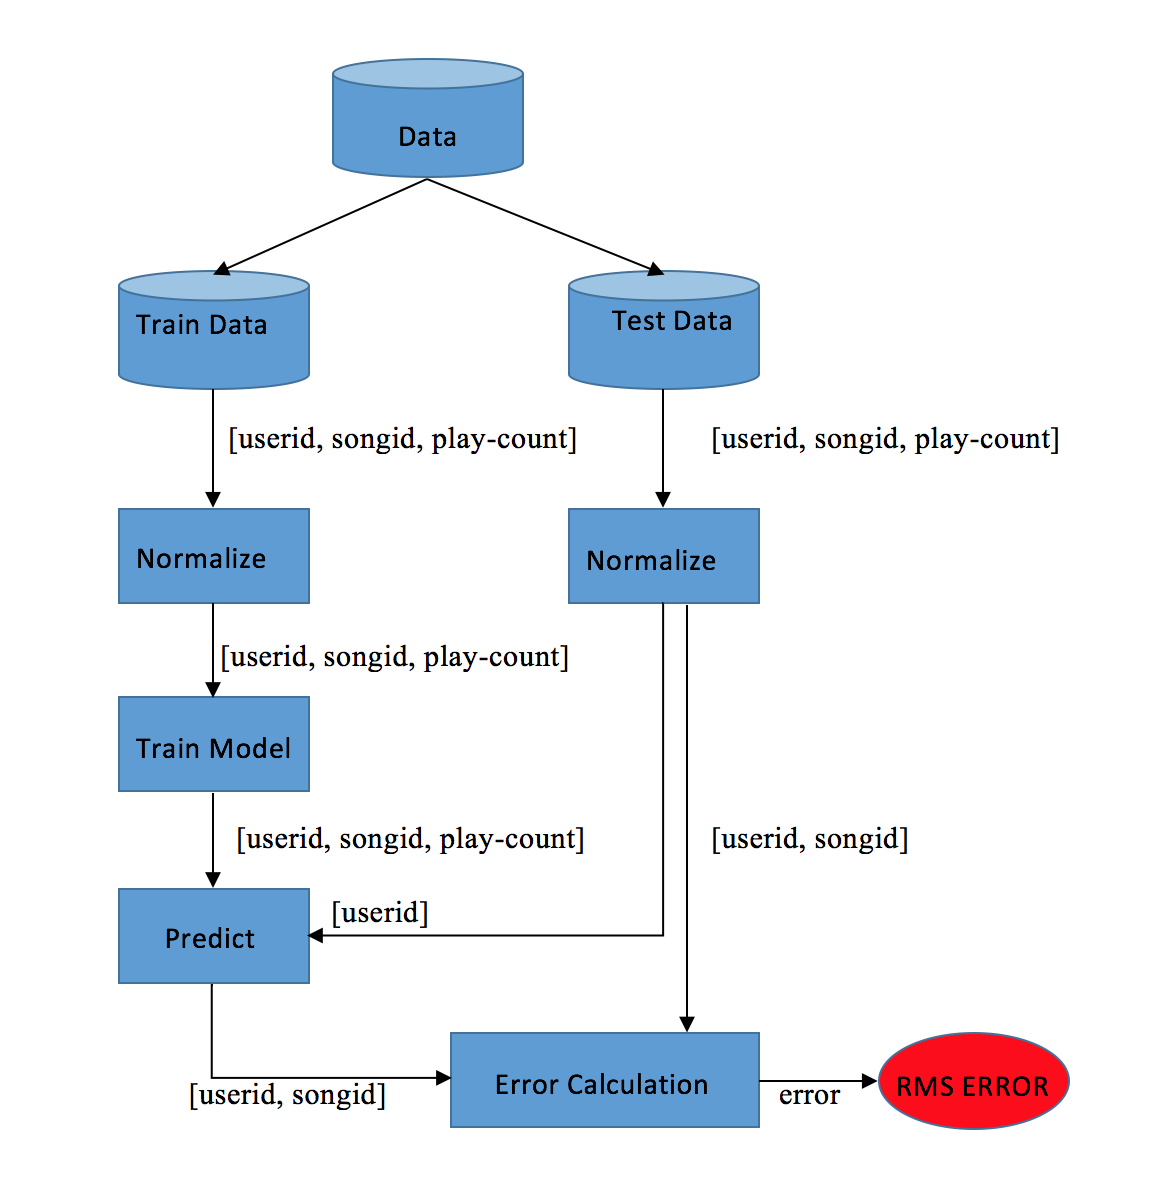
\includegraphics [width =10cm]{Images/SystemStructure.png}
    \caption{Collaborative Filtering model }
\end{figure}


\subsubsection{Content Based Filtering approach}

The second approach is to recommend songs using content-based filtering technique. This is based on the attributes and features of the songs and profile of user preferences. Using the various song attributes like danceability, tempo, energy, timbre, key, loundness, duration, etc. a user profile is built to indicate the type of songs the user likes. This approach will recommend songs to the user which are similar to the songs listened by user in the past. The features of the item would be represented using item presentation algorithms like vector space representation. The profile of the users is based on a weighted vector of item features. The weights denote importance of each feature to the user. The different machine learning algorithms like Bayesian Classifiers, cluster analysis, decision trees, artificial neural networks, etc., can be used to estimate the probability that a user is going like the recommended song. We would be experimenting with many of these machine learning algorithms and select a best algorithm based on evaluating metrics.\\\\
The advantage of content-based filtering approach is that it is user independent, i.e., it does not need to find similarities between different users. It only have to analyze items and profile of the given user. It does not suffer from cold start, i.e., new songs can be recommended before being rated by any users. The disadvantage is that if the songs does not enough attributes and information to discriminate it with other songs, the recommendation will not be precise. If there is not enough information to build a profile for the user, the recommendation could not be done correctly.

\begin{figure}[h]
    \centering
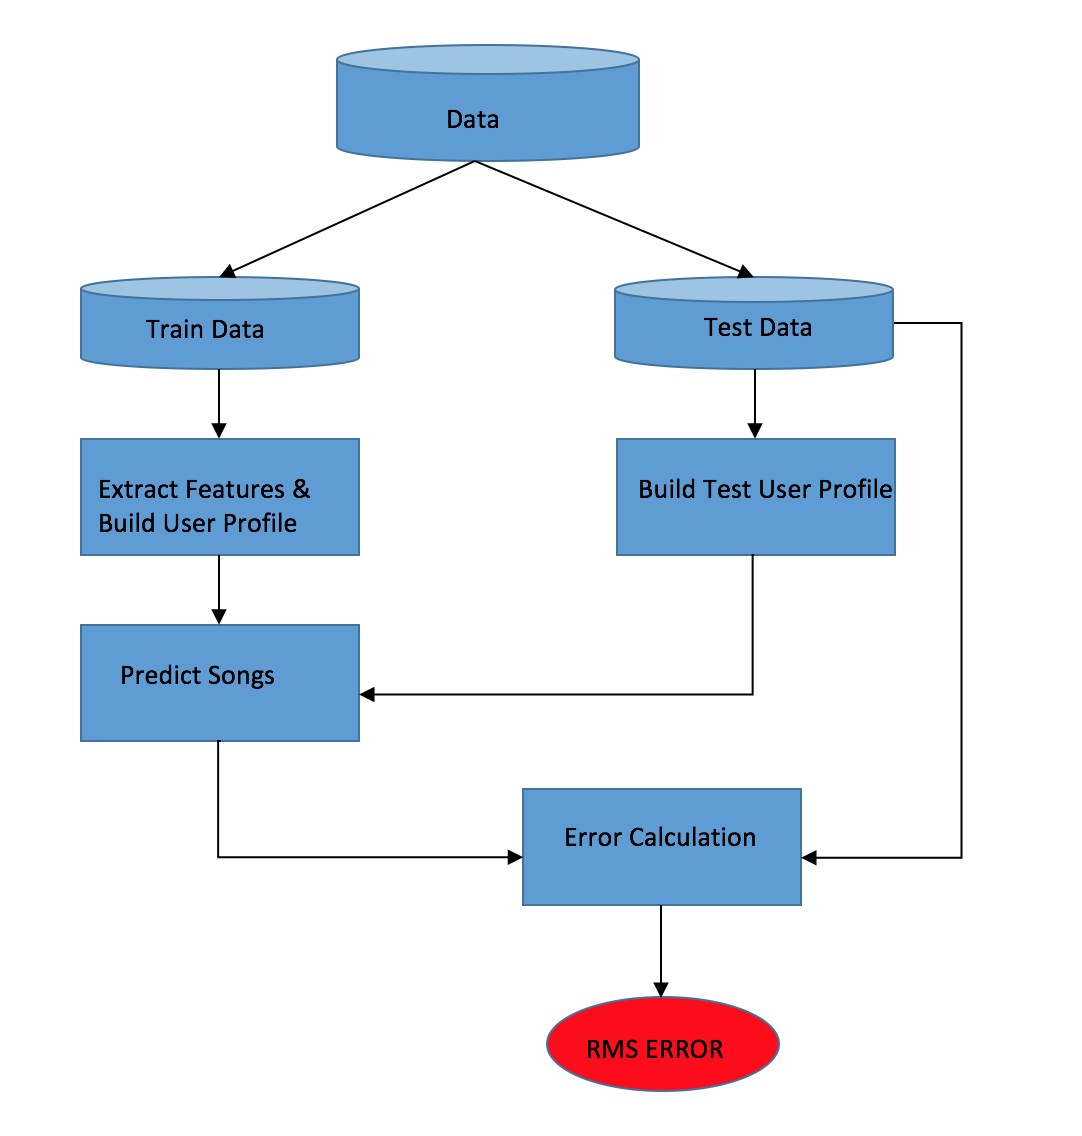
\includegraphics [width =10cm]{Images/ContentBasedFiltering.png}
    \caption{Content Based Filtering model}
\end{figure}

\subsubsection{Hybrid approach}

A more effective recommendation can be done by combining collaborative filtering and content-based filtering. Both of these techniques have some shortcomings as described above, but can be overcome using a hybrid approach. Hybrid approach can be implemented in several ways: by making content-based and collaborative-based predictions separately and then combining them; by adding content-based capabilities to a collaborative-based approach (and vice versa) or by unifying the approaches into one model.\\

This project would make recommendations based on collaborative filter and content-based filter separately and then combine them to give the final recommendations. The collaborative filtering would recommended the songs which have been listened by group of users, but it will not recommend new songs. The content-based filtering approach would be applied to newly released songs which has not yet been listened by a group of users. We will assign a score to the songs recommended by both of these techniques, then sort the songs in decreasing order of their scores and then give the final recommendation. This approach would make sure that the recommendation is for both newly released songs as well as popular listened songs.\\

\begin{figure}[h]
    \centering
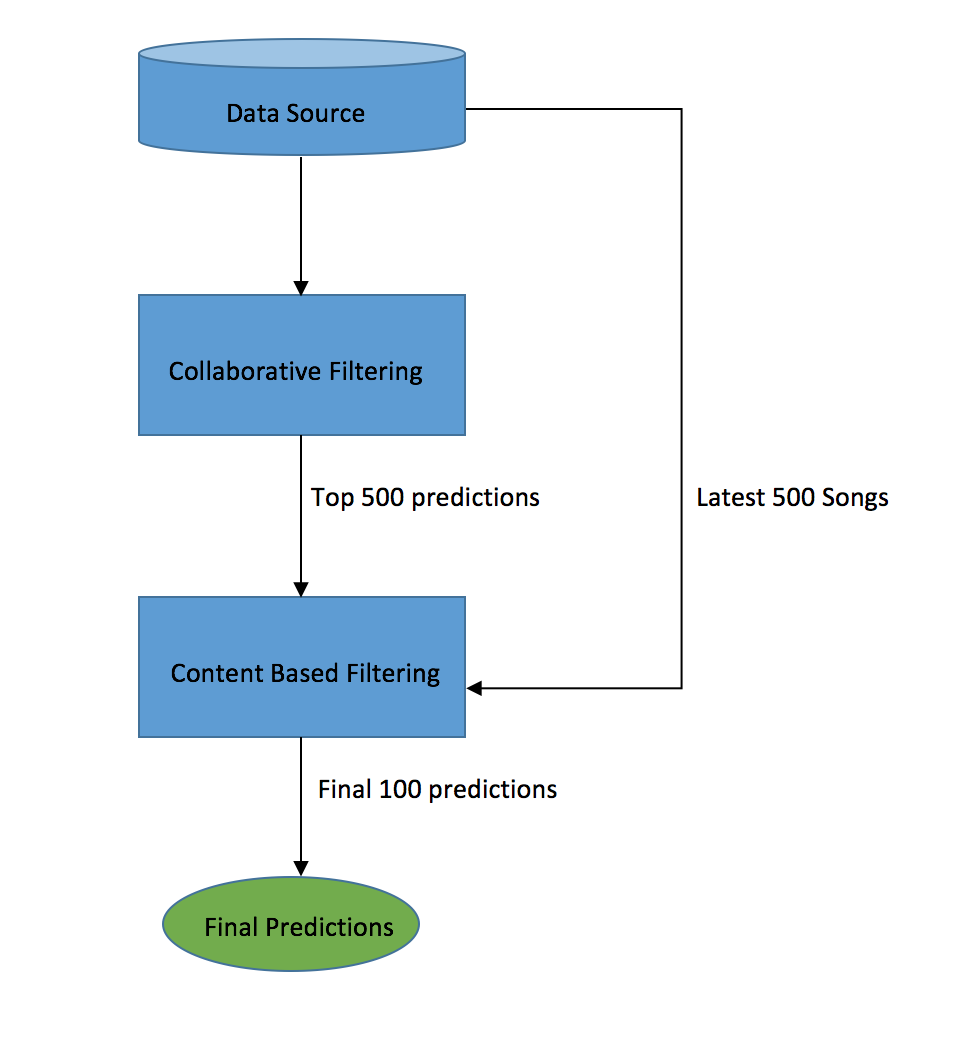
\includegraphics [width =10cm]{Images/HybridStructure.png}
    \caption{Hybrid Music Recommender System}
\end{figure}

\subsection{Building an Automatic Genre Classification System}
A music genre is conventional category that identifies some piece of music as belonging to some stylistic criteria. Automatic Genre Classification is the classification of a given piece of music into its genre using data mining techniques and machine learning algorithms. The music genre classification would be done by building a feature representation of the song followed by a classification system which would predict the genre.\\\\
The various feature classes to represent acoustic and musical aspect of the data are timbre (sound texture), loudness, tempo, danceability, key, energy, duration, artist name, etc. Commonly used classifiers are Support Vector Machines (SVM), k-Nearest-Neighbor (kNN) classifiers, Gaussian Mixture Models, Linear Discriminant Analysis (LDA), etc.\\

\subsection{Dataset Description}
The Million Song Dataset (MSD), is used as the primary dataset for our project. The raw data consisted of listening history of a million users in HD5 format. The dataset consists of the listening history of million users. but we used only a part of the data in our project. The whole dataset is about 280 Gb which consists of 48 million entries in it. We have considered a subset of 1 million entries and we have divided the same into Train and Test data in the ratio of 4:1 for testing and evaluating the accuracy of the system.

The super set consists of 90 attributes, 12 timbre average and 78 timbre covariance. The first value is the year (target), ranging from 1922 to 2011.The songs features are extracted from the The Echo Nest API. We take the average and covariance over all segments, each segment being described by a 12-dimensional timbre vector.

It is a freely-available collection of audio features and metadata for a million contemporary popular music tracks. We would first load the user data and run a collaborative filtering methods on it such as Probabilistic Latent Semantic Analysis. For Collaborative filtering we considered attributes like SongId, UserId and the Play count of the songs.

\begin{center}
\begin{tabular} { |p{4cm}|p{4cm}| } 
\hline \textbf{Type of Data} & \textbf{Number of Records} \\
\hline Number of Songs & 10000 \\
\hline Number of Records  & 1.45 million \\
\hline Train Data & 1.16 million \\
\hline Test Data & 0.29 million \\
\hline
\end{tabular}
\end{center}

This method would predict the songs the user might like. The next step we consider attributes like Dancebility, Loudness, Timbre, SongHotness, ModeofConfidence etc of the songs predicted and train a model using machine learning algorithm such as logistic regression, Support vector machine, Naive Bayes etc and then predict the final recommendations.

\subsubsection{Data Collection and Preprocessing}

Dataset named Million Songs is available here. The whole dataset is about 280GB of which we have considered a subset of 3GB for evaluating the system. We have reduced the dataset by considering less number of attributes from the dataset. Of the total 90 attributes we have considered only 15 attributes. We considered the following attributes for the reduced dataset
\begin{itemize}
    \item Danceability: A number that ranges from 0 to 1, representing how danceable The Echo Nest thinks this song is.
    \item Duration: Length of the song, in seconds.
    \item Energy: A number that ranges from 0 to 1, representing how energetic The Echo Nest thinks this song is.
    \item Key: The key that The Echo Nest believes the song is in. Key signatures start at 0 (C) and ascend the chromatic scale. In this case, a key of 1 represents a song in D-flat.
    \item Loudness: The overall loudness of a track in decibels (dB).
    \item Mode: Number representing whether the song is in a minor (0) or major (1) key. Use this in conjunction with 'key'.
    \item TimeSignature: Time signature of the key.
    \item SongId: Unique Identifier of the song.
    \item UserId: Unique Identifier of the user.
    \item PlayCount: Number of times the song has been played by a particular user.
    \item TrackId: Unique Identifier of the track.
    \item TimbreAverage: Superset has a total of 12 attributes for AverageTimbre. So we have reduced it to a single attribute which is a mean of all the 12 timbre values in the dataset.
    \item ArtistName: Name of the artist of the album.
    \item Title: Title of the song.
    \item Tempo: It gives the number of beats per second of the song.
\end{itemize}
\\\\\\\\\
\subsubsection {Data Cleaning}\\\\\\
The total size of dataset is around 280GB and it is possible to build a model using the whole dataset, but building this model takes approximately close to 16 hours of runtime. So in order to reduce the runtime we considered a subset.\\\\
Since we have considered a subset of data there could be instances where the features of the songs are not available. For these instances we are ignoring the whole song from being considered for the recommendation of the songs.\\\\
The other option we have included is that if a numeric attribute is missing we have considered a mean of the range of values for that attribute. For example, we consider ''Danceability'' attribute whose value ranges between 0 and 1, if its missing we consider 0.5 as the default value of the attribute.\\
\subsubsection {Data Warehouse}
We are considering a dataset for 10000 songs with around 1.45 million entries in the dataset. We have used a CSV (Comma Separated Value) file system to store this data.\\\\ We have considered two files, one for Collaborative Filtering where we consider only three attributes namely UserId, SongId and the PlayCount (TrainTriplets). For Content based filtering we have to consider various features of the song like tempo, timbre etc for which we have used another CSV file. The entries in these files are mapped using SongId.
\newpage
\subsection{Sub-Task}
\subsubsection{Completed Tasks}
\begin{itemize}
    \item \textbf{Recommending popular songs to the user using Collaborative Filtering}\\
    For this task we used Apache Spark model-based collaborative filter which uses Alternating Least Squares (ALS) algorithm to learn the latent factors. We normalized the play-count attribute from the traintriplets, in order to reduce the values to a same scale, we have used min-max normalization which is given by,
    \begin{equation*}
        X = \frac{x_i-min}{max-min}
    \end{equation*}
    
    We ran the ALS algorithm on the traintriplets with normalized play-count to build a model, which was used to predict the songs for the test data.
    
    \item \textbf{Implemented a Genre classifier}\\
    For Genre Classification we extracted various features of songs from MSD. This feature set includes ``Loudness'', ``Tempo'', ``TimeSignature'',``Mode", ``Key'', ``Average Timbre'', ``Duration'' and ``Variable Timbre'', for classifying the songs.\\
    
    We split the data in the ratio of 4:1 for train and test data respectively and run random forest classifier on the train data to build the model. We predict the genre labels for the test-data using this model.
    
    
    \item \textbf{Evaluation of Model-Based Collaborative Filter}
    
    We used the model to predict the songs for a particular user for whom we had the listening history. Then correctness of the model was computed using Root Mean Squared Error. \\\\
    The MSE of the model with different values of regularization parameter, rank are computed and
    tabulated below.
    
    
\begin{center}
\begin{tabular} { |p{2cm}|p{2cm}|p{2cm}| } 
\hline \textbf{Lambda} & \textbf{Rank} &\textbf{MSE} \\
\hline 1.0 & 8 & 15.23 \\
\hline 10.0 & 8 & 16.41 \\
\hline 5.0 & 8 & 12.17 \\
\hline
\end{tabular}
\end{center}

The Mean squared error of the collaborative filter model with testing data is given below in the table.
\begin{center}
\begin{tabular} { |p{4.4cm}|p{2cm}| } 
\hline Mean Squared Error & 12.31 \\
\hline Mean Absolute Error & 2.41 \\
\hline Root Mean Square Error & 3.51 \\
\hline
\end{tabular}
\end{center}
    
    \item \textbf{Evaluation of Genre Classifier}
    
    We used the model to predict the genre of the songs for which we had the genre labels. The model predicted labels were compared with the actual labels to compute the accuracy of the classifier.\\\\
    The accuracy of the genre classifier model using Random forest is show below,

\begin{center}
\begin{tabular} { |p{2cm}|p{3cm}|p{1.5cm}| } 
\hline \textbf{Feature-Id} & \textbf{Feature vector} &\textbf{Accuracy} \\
\hline $F_0$ & genre, track id, tempo, time signature, duration, loudness, key, mode, danceability & 50\% \\
\hline $F_1$ & $F_0$, average timbre, variable timbre & 56\% \\
\hline
\end{tabular}
\end{center}
\end{itemize}


\subsubsection{To-Do Tasks}
\begin{itemize}
    \item Recommending songs to the user using Content based Filtering.
    \item Integrating Content based filtering with Collaborative Filtering to generate a hybrid model for recommendation.
    \item Integration with existing music systems (iTunes, Google music, etc).
    \item Recommending songs based on the category with mood tags such as ``sad", ``happy", ``joyful", ``romantic", etc.\\
\end{itemize}

\subsection{Evaluation}
To evaluate how well our system would perform, we can make use of different metrics like Mean Squared Error, Root Mean Squared Error, precision and recall or DCG. We will split the input data into training set and test set. \\
\begin{equation*}
    RMSE = \sqrt{\frac{1}{n}\sum_{p,q}|{P_{u,v}}- {R_{u,v}}|^2}
\end{equation*}
The test set should be only a small fraction of the complete data. The idea is to hide the test set from the system and see how well the system is able to reproduce it. We will use the training set as input data to the recommender system to build the classifier. The system would then produce the recommendations, which we will compare to what the user actually listened to and use the above mentioned metrics to compute a accuracy of our model.

\section{Key Results}
\subsection{Collaborative Filter}
  For Collaborative Filtering we used Apache Spark model-based collaborative filter which uses Alternating Least Squares (ALS) algorithm. In order to find the right regularization parameter lambda value we run the ALS for different values of Lambda and plot it against the Mean Squared Error for each respectively.We set the rank as 8 and iterate it over 10 times to plot the graph. Thus we get a graph shown in Figure 5. From the figure we can conclude that the Lambda value around 3 has the least Error and gives more accurate recommendations when compared to the rest.
  
\begin{figure}[h]
    \centering
    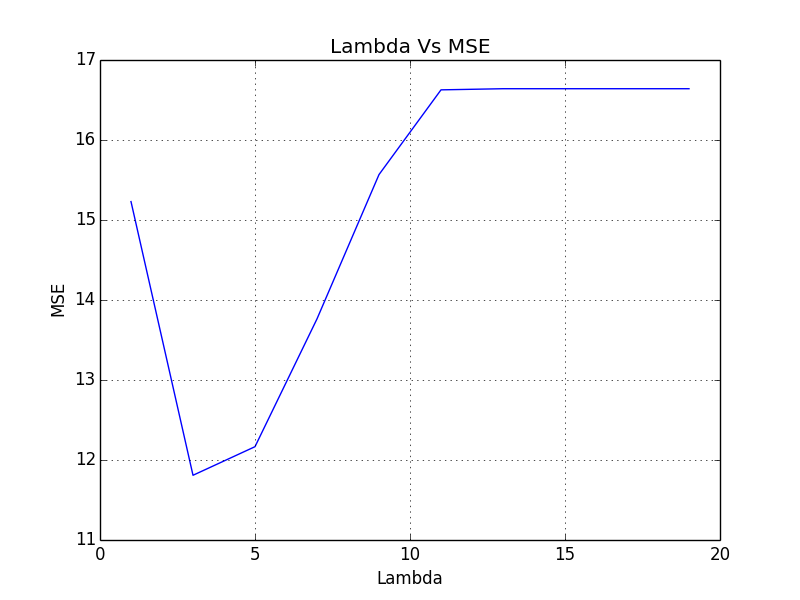
\includegraphics [width =10cm]{Images/RegParam_Collab.png}
    \caption{Effect of Regularization parameter}
\end{figure}

\subsection{Content Filter}

\subsection{Hybrid Filter}
In order to compare the performance of the different techniques we plotted a graph of Recall Vs Number of Song Recommendations.Content Based Filtering offers the least accuracy when it is used without Collaborative filtering. Collaborative Filtering gives a better accuracy than Content Based but it is still low on an absolute scale.
By merging the two techniques we came up with a hybrid model to improve the accuracy of the recommendations. We fed the output of Collaborative Filtering to the Content based Filter to come up with the recommendations which were closer to the user interests. As we can see in the graph the accuracy is slightly improved over collaborative filtering.

\begin{figure}[h]
    \centering
    \includegraphics [width =10cm]{Images/compare.png}
    \caption{Comparing Collaborative filtering, content based filtering with Hybrid filtering}
\end{figure}

\subsection{Genre Classifier}
For Genre Classification we used different classifiers and compared the performance of different techniques. We used various classifiers like Logistic Regression,Decision Tree, Naive Bayes,Random Forest, Support Vector Machines and SVM with boosting. We plotted the Accuracy and Errors of each of the techniques. With this we could conclude that the best technique was to use Random Forest which works on Esemble learning methods. This technique recommended music and had the highest accuracy values as show in the graph.
\begin{figure}[h]
    \centering
    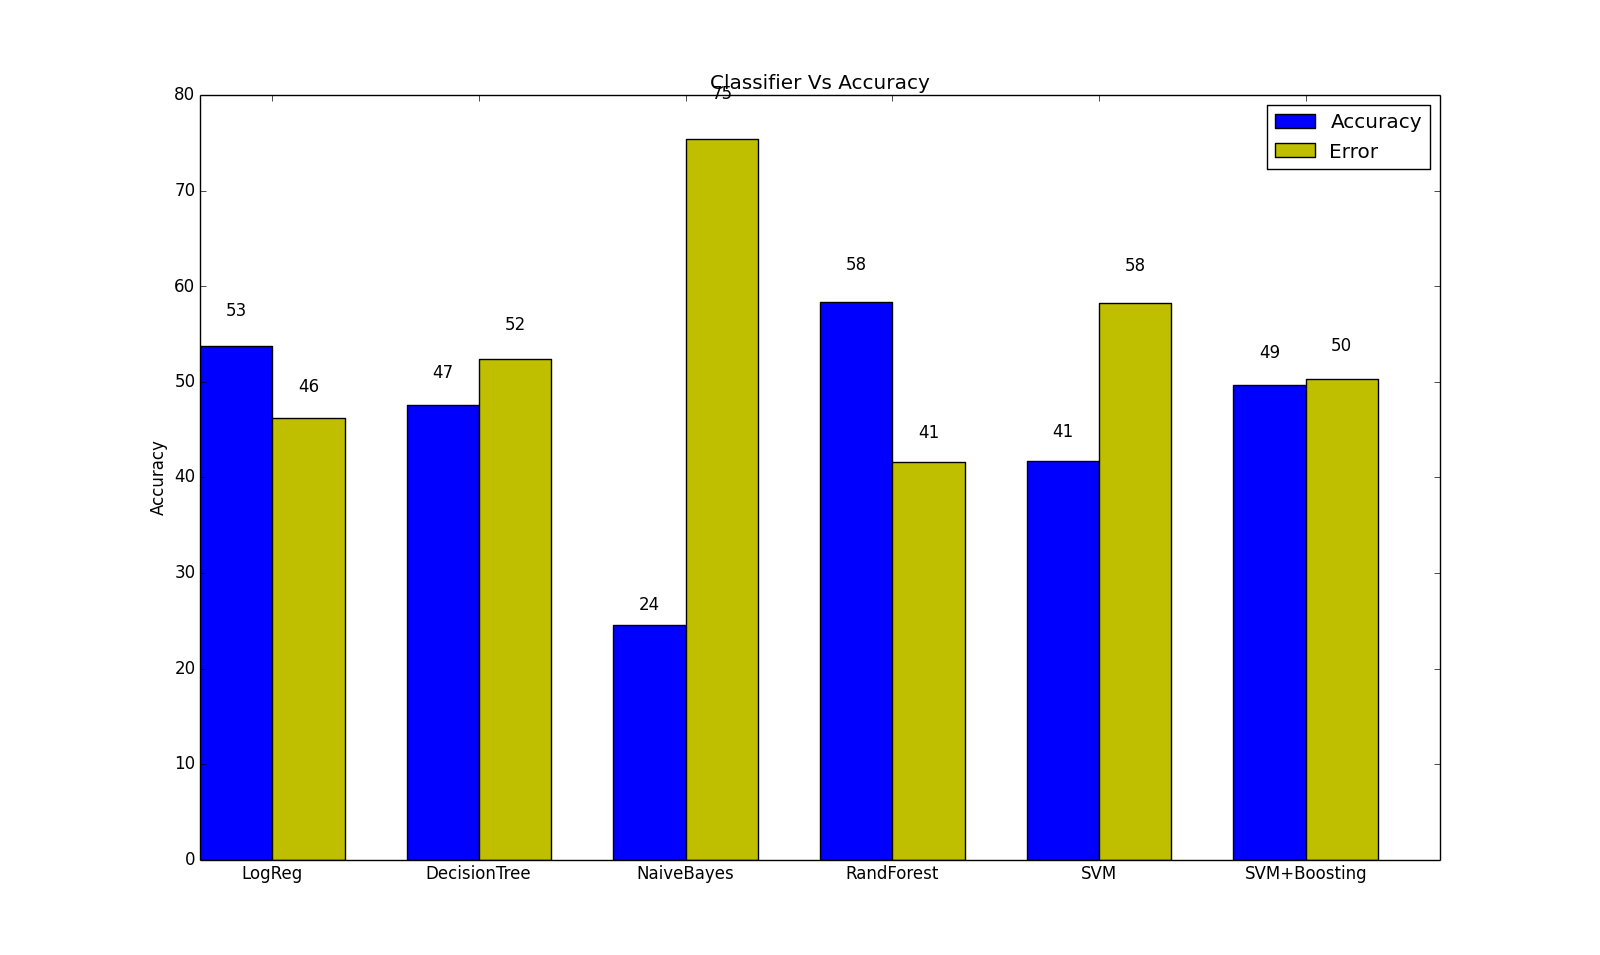
\includegraphics [width =10cm]{Images/Genre_Accuracy.png}
    \caption{Accuracy of Genre classifier with different techniques}
\end{figure}

\begin{figure}[h]
    \centering
    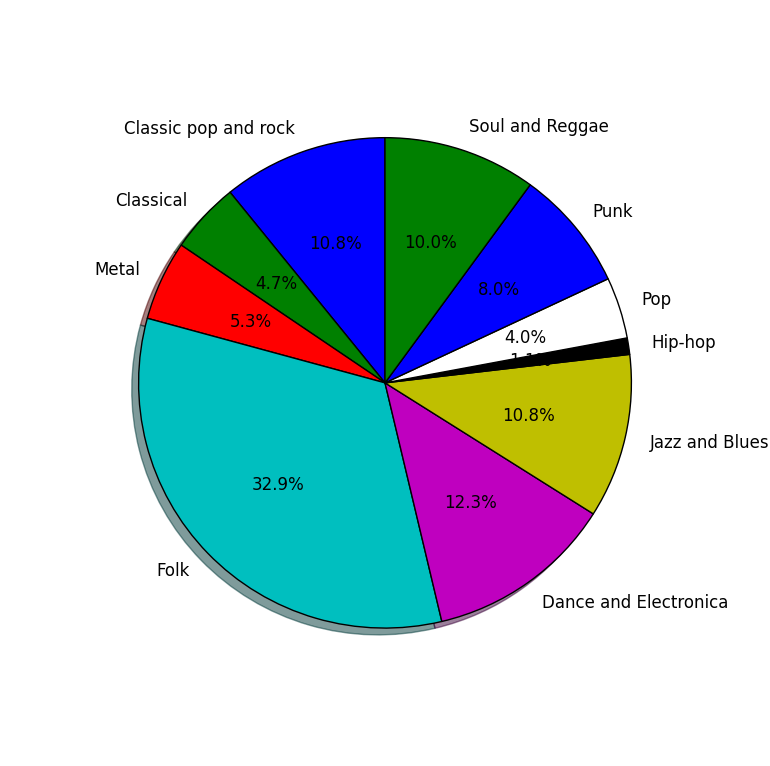
\includegraphics [width =10cm]{Images/GenreDIst.png}
    \caption{Accuracy of Genre classifier with different techniques}
\end{figure}

\section{Future Scope}

\begin{itemize}
    \item Implement Music Recommendation system using Deep learning techniques.
    \item Recommend songs based on what kind of music a user likes to listen during different time periods in a day.
    \item Mood tags ``sad``, ``happy``, ``joyful``, ``romantic``, etc. are not available in MSD. The approach would be to manually tag the songs with the moods and build a model which can be used for recommendation of songs based on moods. \\
    \item Integration with existing music systems(iTunes, Google music, etc). \\
\end{itemize}

\section{Peer Evaluation}

The peer evaluation was done in collaboration with project team working on - `Mining stack overflow data`. Authors: Nikhil Mahendra, Sachin Muralidhara, Aadish, Saurabh sood.\\

The goal of peer review is to help improve classmate's work by pointing out strengths and weaknesses that may not be apparent. During this session we had to answer several questions and few of the interesting ones are listed below.\\

What data is used to train the model for genre Classification? \\

As we know in Million songs dataset, we do not have an explicit attribute genre for all the songs in the dataset. There is a small dataset with genre attributes (the GTZAN dataset). We intend to classify the songs in MSD based on genre using a cross-modal retrieval framework which combines features of lyrics and audio available in MSD. Our likelihood-based training, combining audio sequence features and text features, is done using techniques like Hidden markov model(HMM) and Bag of words model for lyrics of the songs available in MSD.\\

What is unique about our approach in Hybrid recommendation? \\

Popular companies have been using collaborative filtering or content based filtering to come up with the recommendations. We propose a hybrid music recommender system that theoretically integrates collaborative data (rating scores of users) and content-based data (acoustic features of audio signals) to meet the our requirements. To integrate these methods (Collaborative and Content based filtering), we first represent user preferences by using content-based data and then make recommendations in a collaborative way by computing the similarities of the music based user preferences.\\

For this we use a probabilistic generative model, called a three-way aspect model, proposed by Popescul et al. which explains the probabilistic generative mechanism for the observed data (rating scores and acoustic features) by introducing a set of latent variables. As part of the generative mechanism, the model directly represents user preferences (latent favorite genres) estimated statistically with a theoretical proof. This estimation makes the method after predicting unknown rating scores by using content what techniques do we use to generate the recommendations.\\

What are the evaluation metrics? \\

To evaluate the performance of the system, we plan to make use of different metrics like Mean Squared Error, Root Mean Squared Error, precision and recall or DCG. We split the input data into training set and test set. The test set should be only a small fraction of the complete data. The idea is to hide the test set from the system and see how well the system is able to reproduce it. We use the training set as input data to the recommender system.\\

The system would produce the recommendations, which we compare with the user history and use the above mentioned metrics to compute a value. Also we would be comparing the accuracy measure with previously existing systems whose accuracy is expressed in terms of RMS Error.

\section{Conclusions}

In this project, we propose a hybrid model for music recommendation, which combines features from audio and lyrics for the task of music genre classification and recommendation. HMM's, lyrics bag-of-words, and loudness/tempo features would be used. Here we proposed a hybrid music recommender system that ranks musical pieces by comprehensively considering collaborative and content-based data, i.e., rating scores derived from users and acoustic features derived from audio signals.\\

We proposed a probabilistic generative model called a three-way aspect model to create our model which can theoretically explain the generative mechanism for both kinds of the observed data.One possible interpretation of the generative mechanism is that a user stochastically selects a genre according to his or her preferences and then the genre stochastically generates a musical piece and an acoustic feature.\\

Thus the joint probability distribution over users, pieces, and features is decomposed into three independent distributions, which are respectively conditioned by genres.This allows us to incrementally train the aspect model according to the increase in users and rating scores at low computational cost.\\

Thus main gist of the project can be summarized below -\\

\begin{itemize}
    \item From features of audio and lyrics predict the genre of the music which is used for classification and recommendation.
    \item A Hybrid Recommender system which offers more accurate recommendations than existing systems.
    \item Apply Deep Learning techniques for computing the similarity in musicals (Future work).
    \item Compare the accuracy of the the different techniques with few evaluation metrics like RMS error etc.
\end{itemize}

\section{Appendix}
Individual Contributions of the team members are mentioned below.
\begin{itemize}
    \item Collaborative Filtering - Sunil BN
    \item Content Based Filtering - Suresh Kumar
    \item Hybrid Filter - Suresh Kumar
    \item Genre Classifier using Logistic Regression, Decision Trees, Naive Bayes and Random Forest - Sunil BN
    \item Data Visualization - Praveen
    \item Genre Classifier using SVM and boosting - Praveen
    \item Performance Comparison - Praveen
    
\end{itemize}

\begin{figure*}[h]
    \centering
    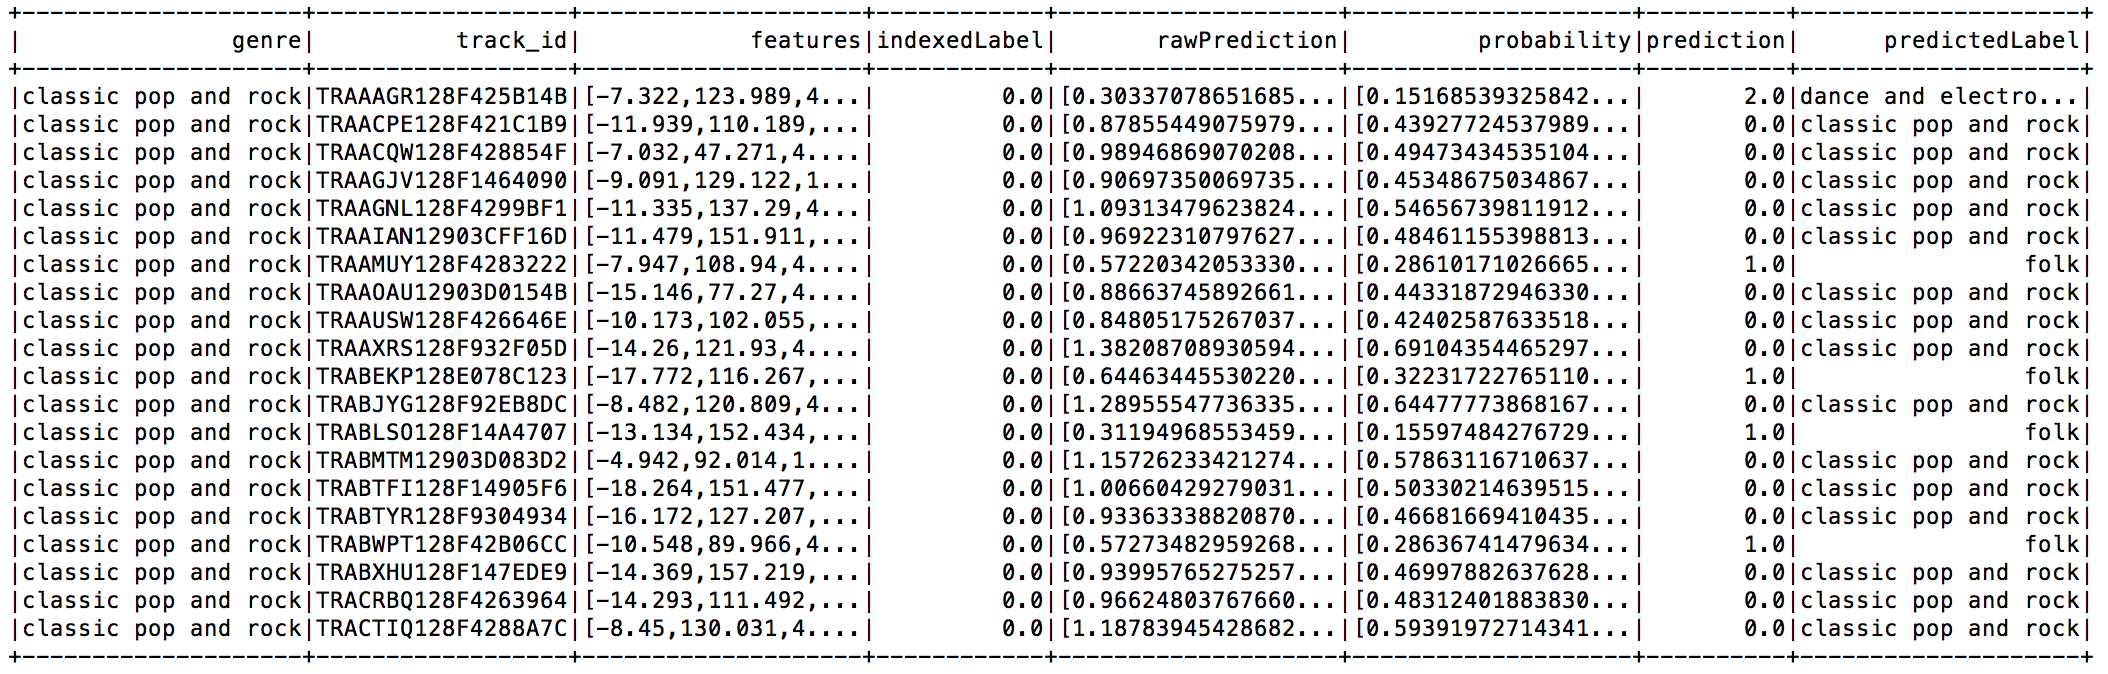
\includegraphics[width=\textwidth,height=\textheight,keepaspectratio]{Images/GenreTop20.png}
    \caption{Accuracy of Genre classifier with different techniques}
\end{figure*}

\begin{figure*}[h]
    \centering
    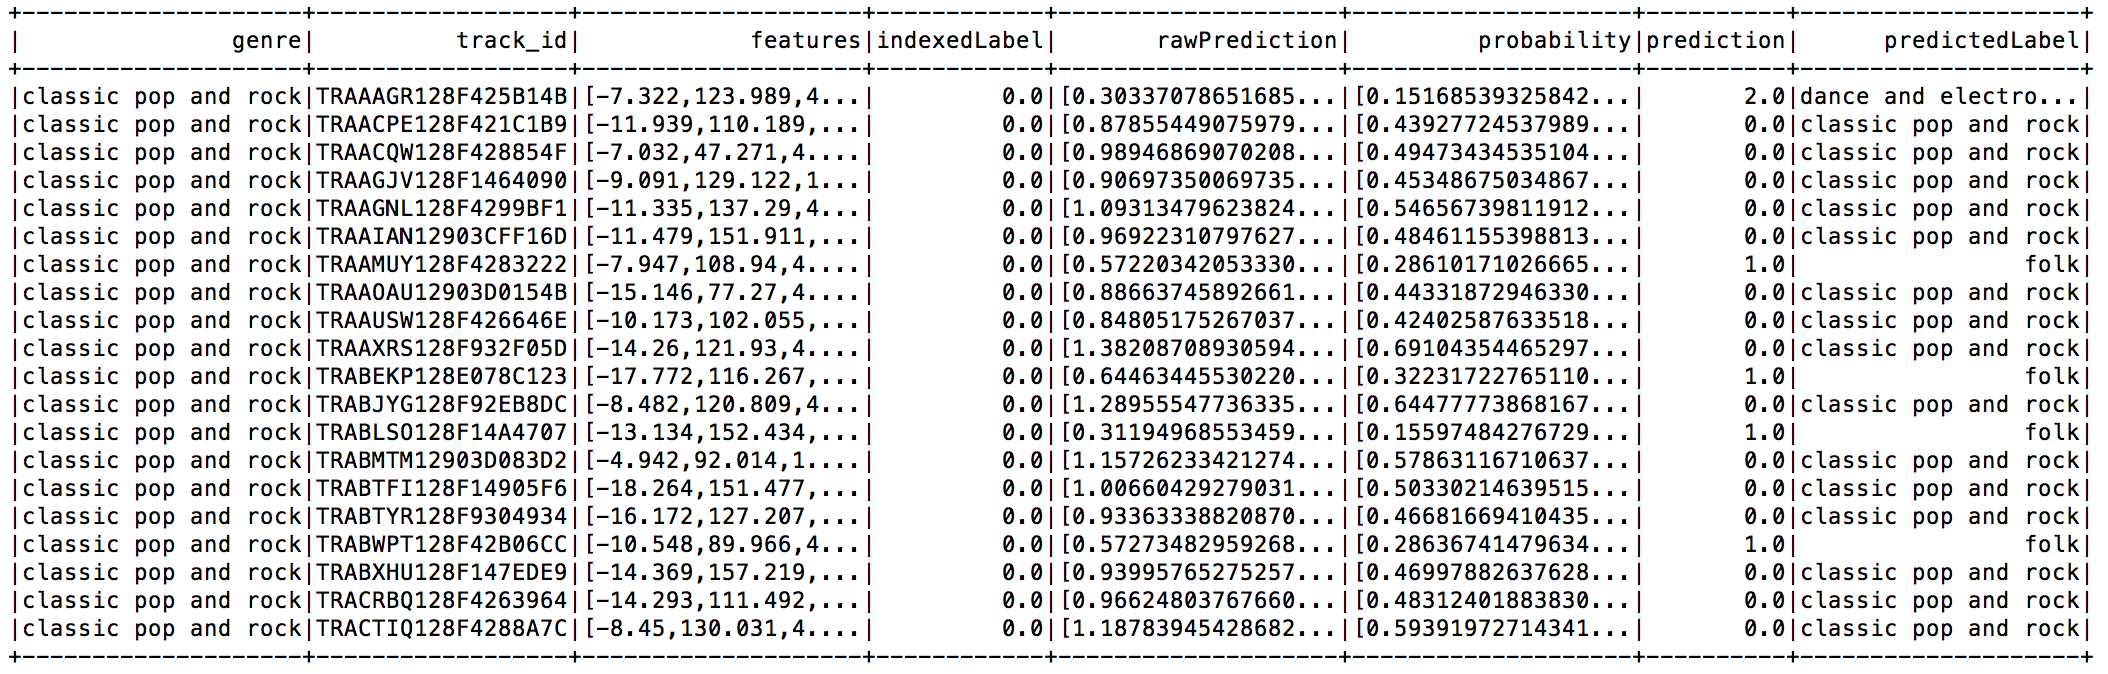
\includegraphics[width=\textwidth,height=\textheight,keepaspectratio]{Images/GenreTop20.png}
    \caption{Accuracy of Genre classifier with different techniques}
\end{figure*}

\begin{figure*}[h]
    \centering
    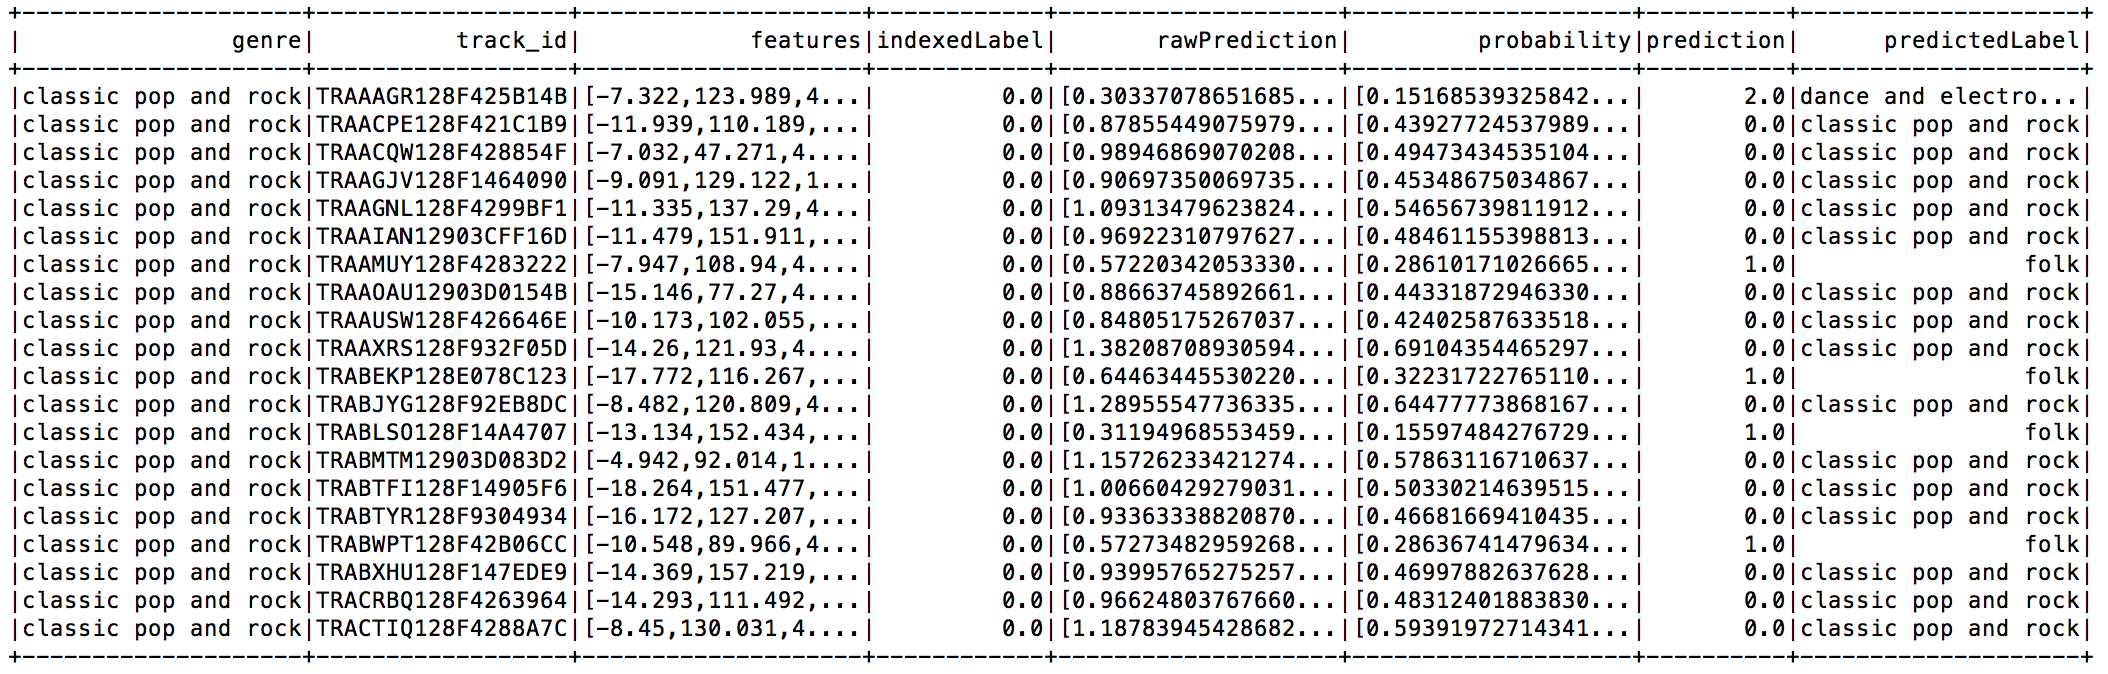
\includegraphics[width=\textwidth,height=\textheight,keepaspectratio]{Images/GenreTop20.png}
    \caption{Accuracy of Genre classifier with different techniques}
\end{figure*}


\nocite{*}

\bibliographystyle{unsrt}
\bibliography{sigproc}

%\balancecolumns % GM June 2007
% That's all folks!
\end{document}
